\section{Definition}

\subsection{Project Overview}

Object recognition is a central topic in the field of computer vision. The numerous applications can be applied in many different domains such as self-driving vehicles environment detection, skin cancer screening or reality augmented tourism.


This project focus on the automatic recognition of flower species from pictures. The potential applications are:

\begin{itemize}
	\setlength\itemsep{1pt}
	\setlength{\parskip}{0pt}
	\setlength{\parsep}{0pt}
	\item population tracking and preservation
	\item crop and food supply management 
	\item toxicity detection 
	\item education
	\item and more...
\end{itemize}

\begin{center}
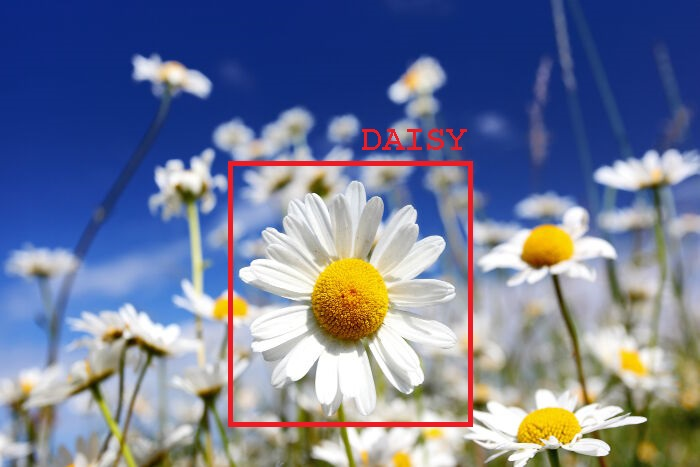
\includegraphics[scale=1.3]{Daisy_detection.jpg}
\captionof{figure}{application example: it's a Daisy!}
\end{center}

Flowers recognitions is already used in mobile applications addressing for example to garden lovers or hitch-hikers \cite{best-apps}. Unfortunately neither the technology or performances of the models used in those products are publicly available. 
However the research work on flower species identification entitled "bi-level co-segmentation method for image classification" from Yuning Chai, Andrew Zimmerman and Victor Lempitsky in 2011 \cite{Chai_BiCos}, demonstrated a robust method involving the combination of image intensive pre-processing and SVM classification training. This work is used as benchmark for this project as specified in the Chapter \fullref{subsec:benchmark}.

\subsection{Problem Statement}

Is it possible to accurately identify the variety of a flower from a picture ?

The today state of the art solution to tackle pictures classification problems is the creation and training of a deep Convolution Neural Network (CNN). The training has to be performed on a dataset  of flower pictures classified by species. 

\subsection{Dataset}

The dataset used in this project is the \lq\lq{}Flowers Recognition Dataset\rq\rq{} of  \href{https://www.kaggle.com/alxmamaev/flowers-recognition}{Kaggle.com}  given by \href{https://alxmamaev.github.io/}{Alexander Mamaev}.\\

The zip archive is 230MB and contains about 4300 flower images (.jpg) classified in 5 classes: Daisy, Dandelion, Rose, Sunflower and Tulip.

\subsection{metrics}

In this project, we aim to build a model able to correctly classify flowers from five different classes. The trivial metrics to evaluate how good the model is at predicting the correct flowers classes is the  \textit{Accuracy} $ACC$ defined as follows: 

\begin{center}

	$ACC = \frac{number \ of \ correct \ predictions}{total \ number \ of \ prediction} \cdot 100$ \cite{sklearn_accuracy}

\end{center}

Moreover, we will use the textit{Classification Cross-Entropy} $H(y, \hat{y})$ in order to evaluate the model progression during the training and save the weights each time a new minima is reached.

\begin{center}
$H(y, \hat{y})=-\sum_{k=1} y_i log(\hat{y_i})$ \cite{cross_enropy}

\end{center}
	